\section{Methodology}
\label{sec:eval:methodology}


% ----------------------- paths to graphics ------------------------

\graphicspath{{6_evaluation/images/}}

% ----------------------- contents from here ------------------------
% 

The focus of this thesis is reducing the size of the data through \textit{whitebox compression} as a data representation model. Therefore, our main evaluation metric will be the \textit{compression ratio}. In terms of benchmarks, we evaluate our system on the Public BI benchmark (Chapter~\ref{ch:pbib}), as we target real, user-generated data rather than synthetic data. The datasets in the benchmark are available as CSV files.

We compare our implementation against two baselines: 1) a real system with enhanced compression capabilities: VectorWise \cite{zukowski2012vectorwise}; 2) a compression estimator model (defined in \ref{subsec:eval:methodology:estimator}). We aim at showing the improvement brought by \textit{whitebox compression} as an enhancement of existing systems: an intermediate data representation layer that remodels the data to create better compression opportunities for existing lightweight methods. For this reason we evaluate \textit{whitebox compression} as an intermediate layer preceding these methods, instead of a stand-alone system. The following sections present the sampling method that we used for the automatic learning process and the methodology for the two baselines.

\iffalse
good words: "prior to"
\fi


% ------- sampling ------- %

\subsection{Sampling}
\label{subsec:eval:methodology:sampling}

The automatic learning process is based on samples. Various characteristics of the data are extracted by analyzing a small subset of rows. Real data may exhibit clustering properties \cite{sidirourgos2013column}, not only when it comes to sequences of numbers but also in terms of pattern locality. Moreover, there are compression techniques that apply to sequences of consecutive numbers (e.g. RLE). To capture these patterns and correctly evaluate the potential for different compression methods, basic single-point sampling is not enough.

To satisfy these requirements we defined a sampling technique that selects blocks of consecutive rows from random uniform points in the dataset. The input parameters are \(count_{total}\)---number of rows in the dataset, \(count_{sample}\)---number of rows in the sample, \(count_{block}\)---number of consecutive rows in a block. We select \(\frac{count_{sample}}{count_{block}}\) random uniform positions in the dataset. From each position we select \(count_{block}\) consecutive rows and add them to the sample. The uniform random selection and the blocks of consecutive rows ensure that we cover the full dataset and capture different local patterns, including sequences of values.

An additional requirement imposed by some pattern detectors is that the sample data fits in memory. To ensure this, our sampling tool can also receive a maximum size in bytes, from which it derives the \(count_{sample}\) and \(count_{block}\) parameters. This calculation is based on estimating the average size of a row.

% TODO-1: [?] image describing the sampling process


% ------- vectorwise baseline ------- %

\subsection{VectorWise baseline}
\label{subsec:eval:methodology:vectorwise}

We chose VectorWise as a baseline for its enhanced compression capabilities. It uses \textit{patched} versions of well known lightweight compression methods: PDICT, PFOR, PFOR-DELTA \cite{zukowski2006super}. \textit{Patching} is an efficient way of implementing compression for skewed distributions, by storing outliers in uncompressed format in order to keep the size of the compressed non-outliers small. VectorWise's compression engine is similar to ours to some extent: the decision upon which compression method to use is based on analyzing a sample of the data. VectorWise handles each column separately and has the capability of independently compressing blocks of data with different methods instead of the full column.

% TODO-1: [?] more details about VectorWise

Our evaluation methodology is based on comparing the size on disk of: 1) uncompressed data (\(size_{uncompressed}\)), 2) blackbox-compressed data with VectorWise (\(size_{blackbox}\)) and 3) whitebox-compressed data further compressed with VectorWise (\(size_{whitebox}\)). From these sizes we can derive the compression ratios:
\begin{align}
\label{eq:eval:vectorwise:ratios}
    \mathit{ratio_{blackbox}} = \frac{size_{uncompressed}}{size_{blackbox}} && 
    \mathit{ratio_{whitebox}} = \frac{size_{uncompressed}}{size_{whitebox}}
\end{align}

\begin{figure}[h]
  \centering
  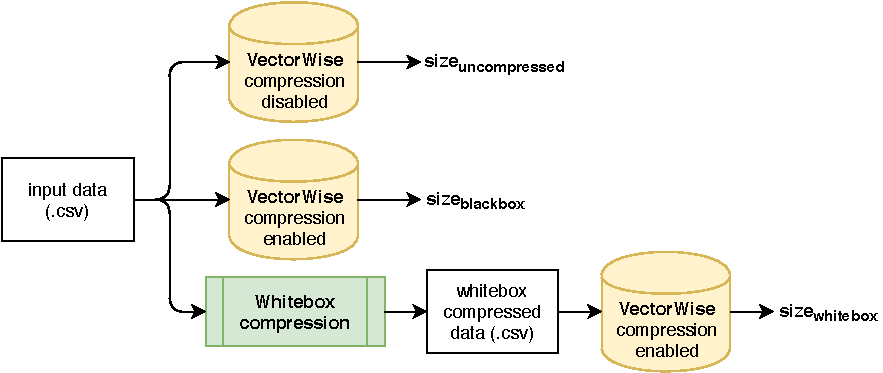
\includegraphics[width={0.98\linewidth}]{baseline_architectures_1-vectorwise_1.pdf}
  \caption{VectorWise evaluation methodology}
  \label{fig:eval:methodology:vectorwisebaseline}
\end{figure}

The evaluation architecture is depicted in Figure~\ref{fig:eval:methodology:vectorwisebaseline}. \(size_{uncompressed}\) is computed by loading the input data into VectorWise with compression disabled. \(size_{blackbox}\) is the size of the data loaded into VectorWise with default compression options (lightweight compression only, LZ4 disabled). \(size_{whitebox}\) is computed by: 1) feeding the input data to the \textit{whitebox compression} engine, resulting in a new representation of it, then 2) loading the new data into VectorWise with the same default compression options. The \textit{whitebox compression} engine learns a compression tree based on a sample and then evaluates it on the input data to materialize the new representation. The additional compression step with VectorWise applies existing blackbox compression schemes on the new representation of the data. The purpose of this 2-step compression process is to isolate and measure the capacity of \textit{whitebox compression} to create better opportunities for existing lightweight compression schemes.

We determine the size of each table by inspecting the raw data files resulted after the bulk loading process. When computing \(size_{uncompressed}\) and \(size_{blackbox}\) we consider the total size of the data files associated with each table, which include the compressed values, exceptions and metadata. For \(size_{whitebox}\) we get the size of all physical columns (including the exception columns) from VectorWise's data files and estimate the size of the metadata in the same way we do in \ref{sub:estimators}~\nameref{sub:estimators}.

In most of the cases VectorWise stores each column in a separate file, allowing us to perform fine grained analysis on the size of individual columns. We noticed, however, that in some cases VectorWise stores multiple columns in the same file. Matching the column names with the data files is not a straight-forward process. The file name has a fixed format which includes the table and column names. However, some characters (mostly non-alphanumeric) tend to be replaced with other (combinations) of characters. We empirically determined some rules for this replacement (e.g. hexadecimal ASCII codes as replacements), but there are also exceptions. Therefore, we implemented a \textit{column-to-file} approximate string matching algorithm based on the Levenshtein distance \cite{levenshtein1966binary} and fuzzy regex matching \cite{pypiregex}---which is out of the scope of this thesis and will not be discussed here.

Individual tables from the benchmark are loaded into VectorWise using the bulk loading utility \verb|vwload| \cite{vwvwload}. We use the \verb|trace point qe82| option to enable/disable compression as indicated in the performance guide \cite{vwperfguide}. The size of each data file is retrieved from the Linux \verb|stat| structure \cite{linuxstructstat}.

We found 2 additional information sources that might be useful for data analysis: 1) the \verb|statdump| command \cite{vwstatdump}---general stats about tables (e.g. histogram) and 2) the compression logs---information from the compression process (e.g. which compression schemes were used). Even though the latter can be useful to understand how VectorWise compresses the data, the logs do not contain any information about which column and which block they refer to, resulting in a mix of information with missing context.  A possible workaround would be to load each column as a separate table, reducing the unknown variables to the block number. This approach is feasible and might lead to interesting comparisons, however we did not proceed with it and we leave it for future work.


% ------- estimator baseline ------- %

\subsection{Estimator baseline}
\label{subsec:eval:methodology:estimator}

We created an alternative evaluation baseline in addition to the VectorWise one: a model which estimates the size of data based on the compression estimators defined in \ref{sub:estimators}~\nameref{sub:estimators}. Its purpose is to simulate a stand-alone \textit{whitebox compression} system, with whitebox versions of existing lightweight compression schemes as leaf nodes in the expression tree. The workflow is similar to the previous one: we compute the 3 sizes from which we derive the compression ratios. The only difference is that VectorWise is replaced by the estimator model, which estimates the size of each column as if it were compressed with whitebox implementations of existing lightweight compression schemes. The final size is the smallest size amongst the ones given by the 4 estimators. The methodology is depicted in Figure~\ref{fig:eval:methodology:estimatorbaseline}.

\begin{figure}[h]
  \centering
  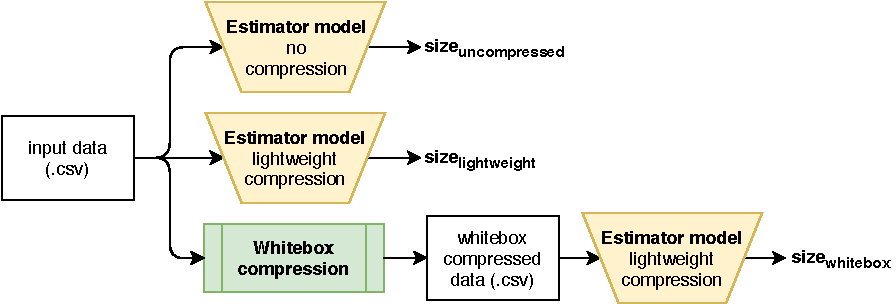
\includegraphics[width={0.98\linewidth}]{baseline_architectures_1-estimator_1.pdf}
  \caption{Estimator evaluation methodology}
  \label{fig:eval:methodology:estimatorbaseline}
\end{figure}

\(size_{uncompressed}\) is computed by estimating the uncompressed size of the input data with the \nameref{subsub:estimator:nocompression}. \(size_{lightweight}\) is the smallest size given by the compression estimators: \nameref{subsub:estimator:dict}, \nameref{subsub:estimator:rle}, \nameref{subsub:estimator:for}, \nameref{subsub:estimator:nocompression}. \(size_{whitebox}\) is computed by first representing the input data through \textit{whitebox compression} and then feeding it to the estimator model.

% ---------------------------------------------------------------------------
% ----------------------- end of thesis sub-document ------------------------
% ---------------------------------------------------------------------------